\newpage
\clearpage

\section{Desenvolvimento do Projeto}
\label{project}

Nos capítulos anteriores, analisamos como as Redes Neurais Convolucionais (CNNs) - Capítulo \ref{cnn} - provocaram mudanças significativas nas abordagens de segmentação, expandindo as possibilidades de obtenção de resultados mais precisos e melhorando o desempenho dos métodos convencionais de segmentação, conforme discutido no Capítulo \ref{segment}.

Entretanto, ainda existem questões não resolvidas relacionadas às potenciais melhorias que modificações específicas nas componentes destas redes podem proporcionar \citep{AsgariTaghanaki2021DeepReview}. Dentre esses componentes, particular atenção é dada às limitações das camadas de \textit{pooling} tradicionais \citep{Liu2019Multi-LevelNetworks, He2015SpatialRecognition}. Estas camadas têm duas tarefas principais: reduzir a dimensionalidade dos dados, a fim de diminuir a carga computacional do modelo, e, simultaneamente, preservar as informações mais relevantes, principalmente as espaciais.

Neste contexto, o objetivo primordial deste trabalho é propor uma nova técnica de \textit{pooling} para CNNs, aplicando testes em CNNs convencionais, mas com ênfase na segmentação semântica com o modelo U-Net. A abordagem proposta visa manter as informações espaciais dos dados de entrada enquanto realiza a necessária redução de dimensionalidade algo que não ocorre com os métodos tradicionais de \textit{pooling}. Os resultados obtidos serão posteriormente comparados com aqueles produzidos pelos métodos de \textit{pooling} comumente utilizados.

Este capítulo trata detalhadamente dos materiais e métodos utilizados para a condução e avaliação da pesquisa, discutidos em profundidade na Seção \ref{project:matmet}. Enquanto a aplicação de métricas específicas para a avaliação dos resultados será discutida na Seção \ref{project:exp_result} e uma breve revisão quanto aos trabalhos relacionados à pesquisa proposta será discorrida na Seção \ref{project:revision}.

Finalmente, vale citar que nesse capítulo será possível encontrar uma apresentação detalhada do novo método de \textit{pooling} proposto e seu impacto na performance das redes de aprendizado profundo.


\subsection{Materiais e Métodos}
\label{project:matmet}
A Seção de Materiais e Métodos busca esclarecer sobre todos os recursos tecnológicos, \textit{hardwares} e abordagens metodológicas que foram empregados para suportar a consecução dos experimentos deste estudo (Seção \ref{project:techard}). Neste contexto, é essencial elucidar acerca da implementação de uma nova técnica de \textit{pooling}, denominada BPCAPooling (Seção \ref{project:bpca}), aplicada em estruturas de CNNs. Além disso, a descrição dos conjuntos de dados utilizados fornece um embasamento sólido para compreender a motivação e a importância dos resultados obtidos ao longo das fases de desenvolvimento, treinamento, validação e teste (Seção \ref{project:dataset}).

Nesta mesma Seção, procura-se detalhar a metodologia e as estratégias adotadas nos experimentos realizados. A abordagem de transferência de aprendizado, em particular, recebe destaque (Seção \ref{project:transf}). Tal técnica envolve a adaptação, ou o chamado \textit{fine-tuning}, de um pré-modelo treinado para operar especificamente na tarefa de interesse, iniciando o processo de aprendizagem a partir de uma configuração pré-definida de pesos, como foi citado na Seção \ref{cnn:augment}.

Além disso, é válida a discussão acerca do procedimento de aumento de dados (Seção \ref{project:augment}), adotado como uma medida para minimizar possíveis vieses nos modelos e potencializar sua capacidade de generalização \citep{Shorten2019ALearning}.

Relacionado aos experimentos, serão expostos os parâmetros-chave selecionados para instanciar e treinar os modelos (Seção \ref{project:params}). Estes parâmetros foram rigorosamente escolhidos de acordo com as melhores práticas.

Por fim, na Seção \ref{project:change_pooling}, abordaremos as respectivas modificações realizadas na camada de \textit{pooling} dos modelos, que foram cruciais para a realização e a validação do experimento. O entendimento dessa sistematização se faz necessário para garantir a replicação das etapas pelos futuros pesquisadores da comunidade científica e proporcionar avanços consideráveis na área de visão computacional.

\subsubsection{Tecnologias e \textit{Hardware}}
\label{project:techard}
Um dos principais recursos tecnológicos utilizados neste trabalho é a linguagem de programação \textit{Python}. Esta linguagem interpretada de alto nível é amplamente reconhecida na comunidade científica, com uma vasta gama de bibliotecas disponíveis que facilitam o desenvolvimento de soluções tanto em aprendizado de máquina e redes neurais profundas, quanto em visão computacional \citep{Millman2011PythonEngineers, Perkel2015Programming:Python}.

Várias bibliotecas complementaram o \textit{Python} no desenvolvimento deste projeto, especialmente aquelas projetadas para auxiliar na implementação de soluções de visão computacional, aprendizado de máquina e redes neurais. Destas, destaco o \textit{TensorFlow} e \textit{Keras}, utilizados juntos como um \textit{framework} para modelar, treinar e testar redes neurais, bem como definir otimizadores, funções de custo e métricas de desempenho \citep{Geron2017Hands-onSystems, Chollet2021DeepPython}. O \textit{OpenCV}, uma biblioteca poderosa para o processamento de imagens e aplicações de visão computacional, também desempenhou um papel crucial na aplicação de filtros de imagens e na realização de testes manuais para afinar os métodos que utilizam aprendizado profundo \citep{Bradski2000TheLibrary.}. Adicionalmente, a biblioteca \textit{Numpy} foi fundamental para realizar cálculos matemáticos e manipulações matriciais \citep{Oliphant2007PythonComputing, VanDerWalt2011TheComputation}.

No que diz respeito ao \textit{hardware} empregado para a pesquisa e desenvolvimento deste projeto, os componentes de \textit{hardware}, tais como as placas de vídeo e os processadores, foram cruciais para o processamento de dados durante as fases de treinamento e validação dos modelos de aprendizado de máquina. Inicialmente, os ensaios foram realizados na plataforma de computação em nuvem Google Colab \citep{Bisong2019GoogleColaboratory}, que disponibilizava uma placa de vídeo Tesla T4 GPU e um processador Intel Xeon CPU. No entanto, devido à limitações de disponibilidade e considerações de custo financeiro, foi realizada a transição para um sistema físico equipado com um processador Intel Core i9-12900F CPU e uma placa de vídeo NVIDIA RTX 4090 GPU, o qual foi considerado para todos os resultados e testes descritos no presente trabalho.

Por fim, é importante ressaltar que todos os métodos desenvolvidos neste projeto com o objetivo de realizar a segmentação semântica serão disponibilizados no repositório Github do autor\footnote{Perfil Github do autor - \url{https://github.com/Lucs1590}}, em conformidade com a licença Apache v2.0 \citep{Licenses}. A intenção é fomentar o crescimento acadêmico e de pesquisa, assim como facilitar futuras melhorias no campo de segmentação com o uso de camadas de \textit{pooling} personalizadas, como a camada BPCAPooling, que é detalhada na Seção \ref{project:bpca}.


\subsubsection{\textit{Block-based Principal Component Analysis Pooling} (BPCA Pooling)}
\label{project:bpca}
A técnica \textit{Block-based Principal Component Analysis} (BPCA) foi introduzida como uma variação do método convencional do \textit{Principal Component Analysis} (PCA) no trabalho de \cite{Salvadeo2011}, propondo um método que inicialmente foi utilizado para a extração de características de imagens como parte de uma \textit{pipeline} de reconhecimento de reconhecimento facial no conjunto de dados \textit{The AR Face Database}\footnote{\textit{AR Face Database Webpage} - \url{https://www2.ece.ohio-state.edu/~aleix/ARdatabase.html}} \citep{MartNez1998TheDatabase} , propondo um método de extração que trouxesse à análise menor custo computacional, redução de dimensionalidade e uma geometria de hiperespaço que fosse mais intuitiva, destacando o diferencial de que com esse método fosse possível preservar a espacialidade da informação.

O método proposto opera por meio da subdivisão de uma imagem em blocos $k \times k$, em que os blocos geralmente possuem tamanhos iguais (por exemplo, $3 \times 3$, $8 \times 8$, etc.). Em seguida, o PCA é aplicado a cada um desses blocos subdivididos. Consequentemente, cada bloco $k \times k$ passa a ter um tamanho reduzido, contendo apenas um subconjunto de pixels com $r$ características (o mesmo numero de blocos). Esse processo pode ser visualizado através da Figura \ref{project:fig:bpca_1}.

\begin{figure}[H]
    \centering
    \caption{Exemplo de aplicação do BPCA.}
    \label{project:fig:bpca_1}
    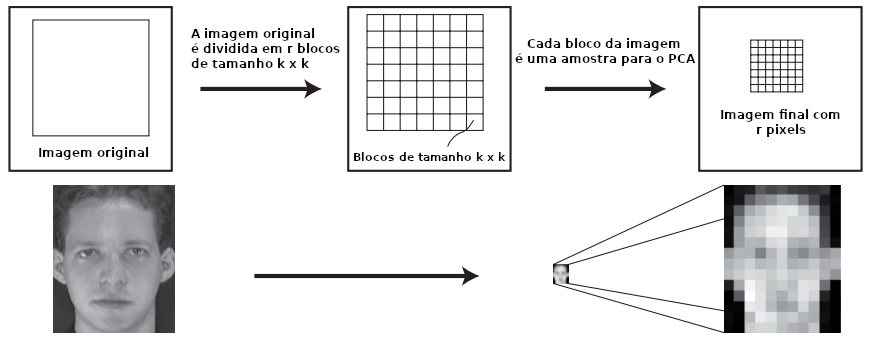
\includegraphics[width=1\textwidth]{recursos/imagens/project/BPCA.png}

    Fonte: retirado e adaptado de \cite{Salvadeo2011}.
\end{figure}

Ao contrário de uma combinação linear simples de amostras distintas, BPCA compõe uma representação organizada, formada por pequenos blocos do mapa de características original, conforme exibido no canto inferior esquerdo da Figura \ref{project:fig:bpca_1}. Esta técnica incorpora a teoria do PCA para realização do mapeamento não supervisionado visando a minimização do erro quadrático médio entre a entrada original e a apresentação projetada. Dessa forma, é possível sintetizar características essenciais da imagem de entrada numa representação compacta de maior relevância contextual \citep{Kuncheva2014PCAData}. Isso permite que a BPCA seja um componente eficaz ao enfrentar grandes volumes de dados, como é comum no âmbito de processamento de imagens.

\paragraph{Funcionamento como \textit{Pooling}}
\label{project:bpca:pooling}
As camadas de \textit{pooling} têm sido eficazes em CNNs para reduzir a dimensionalidade dos dados \citep{Paul2019DimensionalityPooling}. Neste trabalho, a inovação proposta é a aplicação da técnica BPCA como uma camada de \textit{pooling} - sendo nomeada de BPCAPooling - não mais para extração de características, conforme proposto originalmente por \cite{Salvadeo2011}, mas como uma estratégia para preservar a espacialidade da informação entre as camadas convolucionais, associada ao benefício proposto pela técnica de minimização do erro quadrático médio entre a entrada e saída como uma camada de \textit{pooling}.

Essa camada de \textit{pooling} segue o processo original do BPCA, onde são extraídas informações principais de cada bloco, reduzindo a dimensionalidade dos dados e preservando características relevantes. Além disso, o método foi aprimorado pela normalização dos blocos utilizando média ($\mu$) e desvio padrão ($\sigma$). Na sequência, é aplicada a técnica de \textit{Singular Value Decomposition} (SVD) para extrair os componentes principais ($\text{{pca\_components}}$), como explicado na Seção \ref{deep:feature_extraction:pca}, e, finalmente, os blocos são transformados por meio da projeção nesses componentes selecionados. O resultado é um mapa de características menor em tamanho, porém, preservando informações essenciais ao concatenar os blocos transformados.

A formulação matemática do processo realizado pela camada de \textit{pooling} BPCAPooling pode ser representada pela Equação \ref{project:eq:bpca}:

\begin{equation}
    \label{project:eq:bpca}
    \begin{split}
        Y_{i,j,k} &= \text{BPCAPooling}(X_{i',j',k'}) \\
                  &= \text{reshape}\left(\text{SVD}\left(\frac{{X - \mu}}{{\sigma}}\right) \cdot \text{pca\_components}\right),
    \end{split}
\end{equation}
onde $X$ é a imagem de entrada com $i'$ como altura de entrada, $j'$ como largura de entrada e $k'$ como número de canais de entrada; e $Y$ é a imagem de saída, com $i$ representando altura de saída, $j$ como largura de saída e $k$ como profundidade de saída (ou seja, o número de canais). Aqui, $\text{reshape}$ reorganiza os blocos transformados para uma estrutura de saída apropriada, $\text{SVD}$ representa a decomposição em valores singulares dos blocos normalizados, $\mu$ é o vetor médio dos blocos extraídos, $\sigma$ é o vetor de desvio padrão dos blocos extraídos, e $\text{pca\_components}$ é uma matriz contendo os primeiros componentes principais selecionados.

Essa formulação matemática descreve o processo de \textit{pooling} realizado pela camada BPCAPooling, que extrai informações relevantes dos blocos de entrada, reduzindo sua dimensionalidade e preservando características importantes para o aprendizado eficiente da rede neural convolucional.

Quando se trata de complexidade em notação Big O, uma forma de classificar o quanto a função é escalável, pode-se dizer que recebe a notação de ordem $O(mnp^2 + p^3)$ no pior caso. Isso se dá visto que o algoritmo BPCA, constituinte do BPCAPooling passa pelos processos de divisão dos blocos ($p^2$ para cada elemento da imagem de tamanho $m$ e $n$) e a decomposição em valores singulares (operação cúbica em $p$), sendo $m$ e $n$ as dimensões da imagem, e $p$ a profundidade dos blocos. Esse desempenho assinala um compromisso entre a eficiência computacional e a capacidade de extração de características relevantes, demonstrando a relevância do BPCAPooling no contexto da aprendizagem profunda.

Em suma, a camada de BPCAPooling emerge como uma proposta inovadora para aprimorar a atuação das redes neurais convolucionais ao lidar com tarefas de segmentação semântica. Ao incorporar a técnica de BPCA, essa camada de \textit{pooling} permite que a informação espacial seja preservada na passagem entre as camadas convolucionais, mantendo simultaneamente uma redução de dimensionalidade efetiva dos dados. Com seu mecanismo eficiente de extração de características cruciais, o BPCAPooling demonstra uma inovação para auxiliar aos modelos de aprendizado profundo, abrindo caminho para futuras investigações e desenvolvimentos com foco em técnicas de \textit{pooling}.

\subsubsection{Conjuntos de Dados}
\label{project:dataset}
Os conjuntos de dados selecionados para esta pesquisa são essencialmente de duas categorias distintas. Dois deles - CIFAR100 e \textit{Food}-101 - foram empregados especificamente para o treinamento, teste e validação voltados exclusivamente à classificação de imagens \citep{Krizhevsky2009LearningImages, Bossard2014Food-101Forests}.

Nessa configuração, os modelos de classificação foram treinados para atribuir um rótulo a cada imagem, identificando o objeto de interesse sem foco na sua localização ou delimitação por caixas. Em outras palavras, o objetivo foi reconhecer a presença de um objeto em particular na imagem inteira, sem segmentar ou isolar essa entidade \citep{Viitaniemi2008TechniquesSegmentation}.

Por outro lado, um terceiro conjunto de dados - que será detalhado na Seção \ref{project:dataset:pets} - foi preparado especificamente para treinar e validar modelos de segmentação semântica. Este conjunto de dados inclui máscaras que mapeiam a localização dos objetos de interesse em todos os pixels da imagem de entrada.

O emprego desses conjuntos diversificados de dados permite comparar e contrastar a eficácia de diferentes abordagens de segmentação e classificação no campo da visão computacional. Também permite avaliar como esses diferentes métodos respondem a variações nas características dos dados.

As Seções \ref{project:dataset:cifar} e \ref{project:dataset:food101} a seguir detalharão mais apropriadamente os conjuntos de dados utilizados para os experimentos de classificação, e descreverão como foram utilizados no escopo desta pesquisa.

\paragraph{\textit{Oxford-IIIT Pets}}
\label{project:dataset:pets}

O conjunto de dados \textit{Oxford-III Pets} \footnote{Conjuntos de dados \textit{Oxford-III Pets} - \url{https://www.robots.ox.ac.uk/\%7Evgg/data/pets/}} \citep{Parkhi2012CatsDogs} é um composto majoritariamente de exemplos de gatos e cachorros. Esse \textit{dataset} possui cerca de $200$ exemplos para $37$ classes diferentes, resultando no total de $7.349$ amostras. Essas classes é identificada pela raça do animal de estimação em questão, mas cada uma dos registros nesse conjunto de dados trás consigo o nome da imagem, o rotulo baseado na raça, a espécie (gato ou cachorro), a imagem com o animal e uma mascara de características com o fundo, contorno e animal mapeados cada um de uma cor, como representado pela Figura \ref{project:fig:dataset:pets_1}.

\begin{figure}[H]
   \centering
   \caption{Exemplo de exemplo com mascara de características.}
   \caption{Segmentação semântica.}
   \label{project:fig:dataset:pets_1}
    \begin{subfigure}[t]{0.5\textwidth}
        \centering
        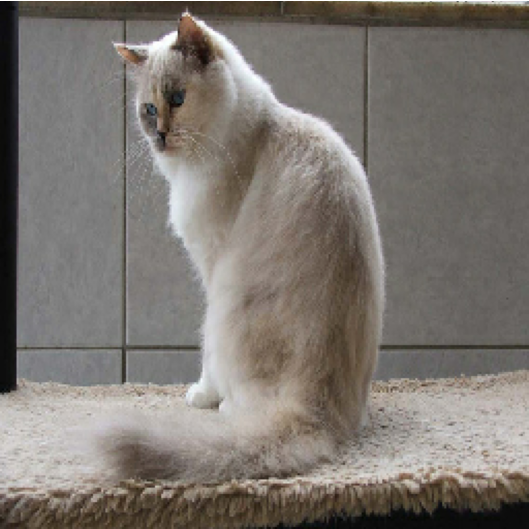
\includegraphics[width=1\linewidth]{recursos/imagens/project/pets_ori.png}
        \caption{Imagem original do animal de estimação.}
        \label{project:fig:dataset:pets_1.1}
    \end{subfigure}%
    ~ 
    \begin{subfigure}[t]{0.5\textwidth}
        \centering
        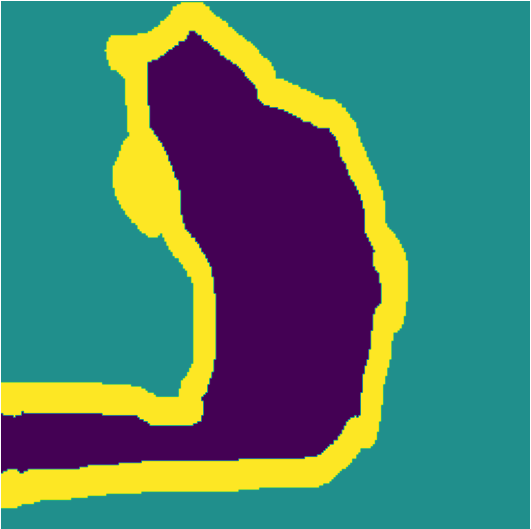
\includegraphics[width=1\linewidth]{recursos/imagens/project/pets_mask.png}
        \caption{Máscara com fundo em verde, contorno em amarelo e animal em roxo.}
        \label{project:fig:dataset:pets_1.2}
    \end{subfigure}%

    Fonte: retirado e adaptado de \cite{Parkhi2012CatsDogs}.
\end{figure}

Vale dizer que originalmente essas amostras estão separadas entre $3.669$ ($49,925\%$) para a etapa de teste e $3.680$ ($50,074\%$) para a etapa de treinamento, todavia nos testes realizados foi utilizado também um conjunto de dados voltado para validação, o qual foi extraído a partir do \textit{dataset} de teste, sendo assim para o presente trabalho a divisão passou a ser de $669$ exemplos para teste, 3.000 amostras para validação e 3.680 instancias para treino, levando em conta os conceitos tratados na Seções \ref{deep:train} e \ref{deep:test}.

É relevante salientar que as imagens do conjunto de dados original são tridimensionais, ou seja, cada amostra inclui informações dos canais de cores vermelho, verde e azul. Já as máscaras são unidimensionais, apresentando um mapa de valores singulares para representar as regiões de interesse baseadas na imagem original. Os valores numéricos nas máscaras correspondem ao fundo, à borda ou ao animal.

Vale observar que diferentemente de muitos outros conjuntos de dados de imagem \citep{Bossard2014Food-101Forests}, o \textit{Oxford-III Pets} não apresenta dimensões padronizadas para suas amostras, todavia no atual trabalho houve uma alteração nesse aspecto, em que foram aplicadas duas técnicas, além da técnica de aumento de dados que será discutida na Seção \ref{project:augment}, em todos os exemplos do conjunto de dados. Sendo que a primeira técnica aplicada foi a padronização tanto imagens originais, quanto das mascaras, em relação às suas dimensões, em que ambas passaram a ter o valor de $256 \times 256$, que é o um valor comumente utilizado na área de imagens para substanciar as características da mesma \citep{Lee1983DigitalFilter}.

Além disso, foi realizada uma normalização dos valores do conjunto de dados. Todas as imagens e máscaras foram normalizadas para um intervalo de $0$ a $1$, conforme a Equação \ref{project:eq:dataset:pets_1}. Para a máscara, essa normalização foi conduzida subtraindo-se um valor unitário de cada pixel, transformando assim o intervalo de valores de $0$ a $1$, conforme a Equação \ref{project:eq:dataset:pets_2}.

\begin{equation}
    \label{project:eq:dataset:pets_1}
    \text{imagem de entrada normalizada}_{(i,j,k)} = \frac{\text{imagem de entrada}_{(i,j,k)}}{255}
\end{equation}

e

\begin{equation}
    \label{project:eq:dataset:pets_2}
    \text{mascara de entrada normalizada} = \text{mascara de entrada} - 1,
\end{equation}
onde $(i,j,k)$ representa as coordenadas de altura, largura e canal, respectivamente.

Por fim, é relevante ressaltar que esse conjunto de dados se mostra adequado para o treinamento em segmentação semântica, uma vez que conta com todos os dados devidamente rotulados, proporcionando um cenário propício para esse propósito. O resultado gerado por essa abordagem será um mapa de características, ilustrado de forma análoga ao apresentado na Figura \ref{project:fig:dataset:pets_1.2}.

\paragraph{CIFAR 1O0}
\label{project:dataset:cifar}
O conjunto de dados CIFAR-100 \footnote{Conjuntos de dados CIFAR-10 e CIFAR-100 - \url{https://www.cs.toronto.edu/~kriz/cifar.html}} \citep{Krizhevsky2014TheDataset} é composto por um total de $60.000$ imagens, cada uma com dimensões de $32 \times 32$ pixels. Estas imagens são categorizadas em $20$ \quotes{superclasses}, cada uma contendo $5$ \quotes{classes finas}.

De maneira geral, o \textit{dataset} possui $100$ classes, com $600$ amostras em cada classe. Cada exemplo neste conjunto de dados é rotulado com uma \textit{superclass}, que representa uma categoria mais abrangente (como "veículo"), e uma \textit{fine class}, que representa uma categoria mais específica (como \quotes{bicicleta}, \quotes{ônibus}, etc.). Alguns exemplos dessas amostras podem ser visualizados na Figura \ref{project:fig:dataset:cifar}.

\begin{figure}[H]
    \centering
    \caption{Exemplos de amostras do conjunto de dados CIFAR-100.}
    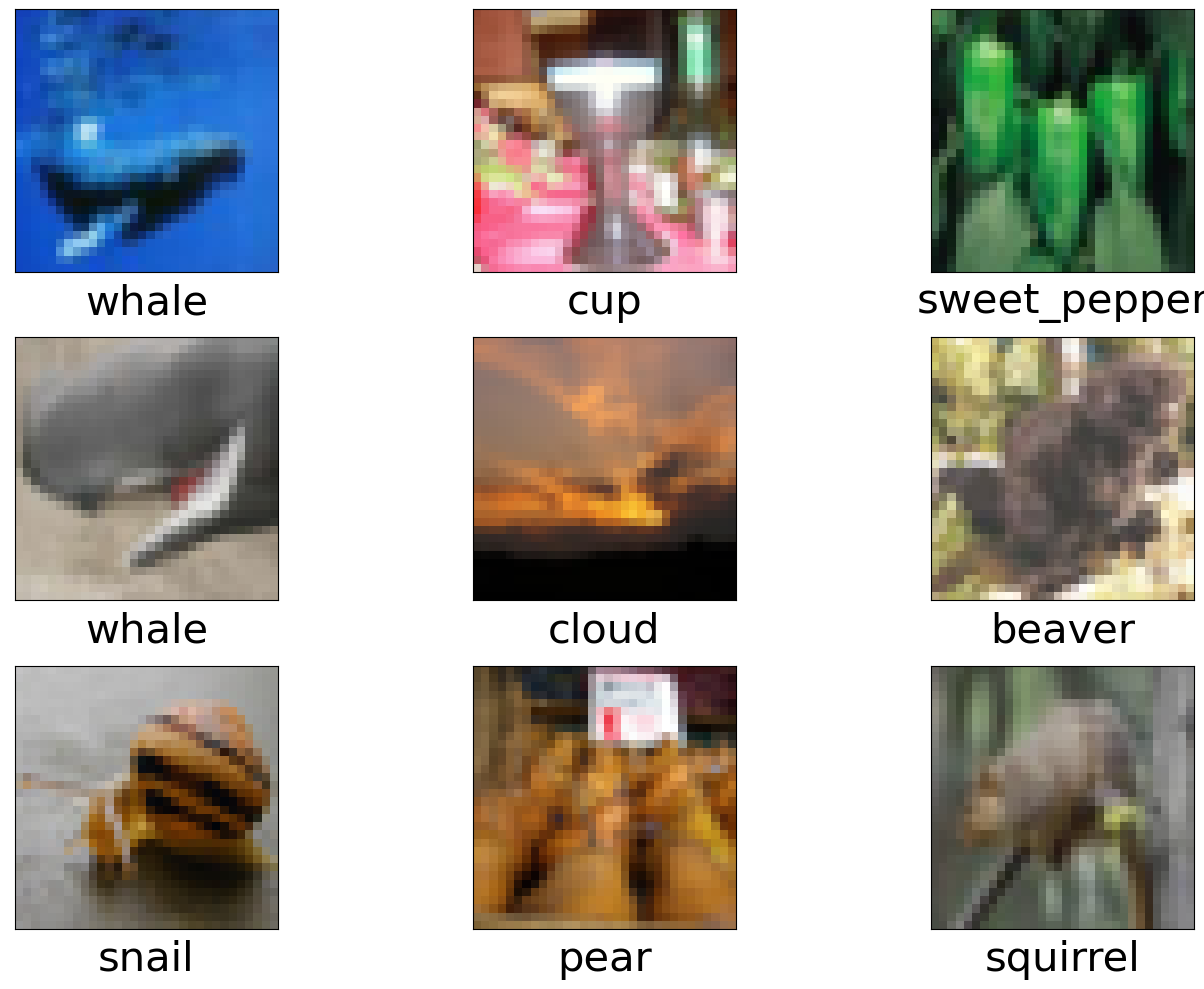
\includegraphics[width=1\textwidth]{recursos/imagens/project/cifar100v2.png}
    \label{project:fig:dataset:cifar}

    Fonte: retirado e adaptado de \cite{Krizhevsky2014TheDataset}.
\end{figure}

Em contraste com a configuração original proposta por \cite{Krizhevsky2014TheDataset}, dividimos o conjunto de dados em $83,33\%$ para treinamento, $11,66\%$ para validação e $5\%$ para teste, visando evitar qualquer viés nos resultados, conforme recomendado por \cite{Domingos2012ALearning}. Além de aplicar um processo de normalização das amostras, deixando o valor de todos os pixels das amostras entre o domínio de $[0, 1]$, com um processo muito semelhante ao da Equação \ref{project:eq:dataset:pets_1}.

Finalmente, vale citar que todas as imagens do conjunto de dados se encontram rotuladas e prontas para serem usadas na tarefa de classificação.

\paragraph{\textit{Food}-101}
\label{project:dataset:food101}
O conjunto de dados \textit{Food}-101 \footnote{Conjunto de dados \textit{Food}-101 - \url{https://data.vision.ee.ethz.ch/cvl/datasets_extra/food-101/}} \citep{Bossard2014Food-101Forests} foi empregado como um segundo conjunto de dados para a classificação de imagens neste trabalho. Este \textit{dataset} contém $101.000$ imagens, originalmente com uma resolução de $512 \times 512$ pixels, no entanto, para otimizar o processamento do modelo e manter a representatividade da amostra, essas imagens foram redimensionadas para $224 \times 224$ pixels.

Ao contrário do conjunto CIFAR-100, que abrange classes mais generalistas (vide Seção \ref{project:dataset:cifar}), o conjunto de dados \textit{Food}-101 se concentra exclusivamente em classes relacionadas à alimentação. Ele é composto por $101$ classes (por exemplo, \quotes{pizza}, \quotes{bruscheta}, entre outros), cada uma com $1.000$ amostras. Alguns exemplos dessas classes podem ser visualizados na Figura \ref{project:fig:dataset:food}.

\begin{figure}[H]
    \centering
    \caption{Exemplos de amostras do conjunto de dados \textit{Food}-101.}
    \label{project:fig:dataset:food}
    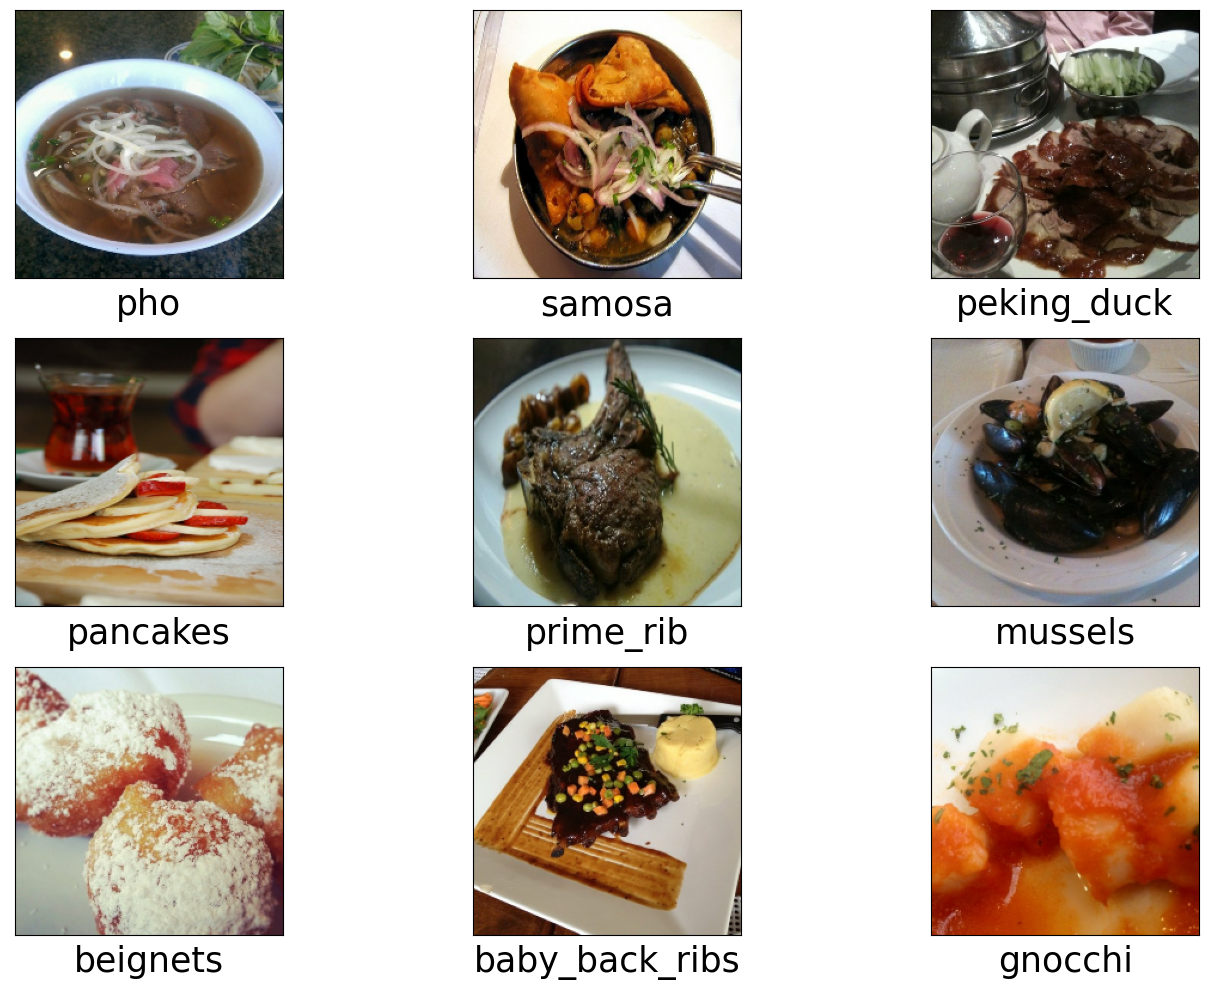
\includegraphics[width=1\textwidth]{recursos/imagens/project/food101v2.png}

    Fonte: Adaptado de \cite{Bossard2014Food-101Forests}.
\end{figure}

Adicionalmente, houve uma reorganização do conjunto de dados em relação à sua configuração original, sendo que $75\%$ das amostras foram designadas para o conjunto de treinamento, $17,5\%$ para validação e $7,5\%$ para teste. Além disso, foi aplicado um pré-processamento de normalização, conforme representado na Equação \ref{project:eq:dataset:pets_1}, com o intuito de reduzir o viés do modelo durante o treinamento \citep{Shorten2019ALearning}.

É importante ressaltar que o conjunto de dados \textit{Food}-101 também foi empregado no processo de classificação de imagens. Ele atua como um conjunto alternativo, permitindo demonstrar a capacidade de generalização do modelo e da técnica utilizada em diversos cenários. Devido ao seu tamanho, uma amostra do \textit{dataset} \textit{Food}-101 contém aproximadamente dezesseis vezes mais informações do que uma amostra do CIFAR-100, o que proporciona uma maior riqueza de detalhes e complexidade para o treinamento e validação do modelo.

\subsubsection{Transferência de Aprendizado}
\label{project:transf}
A técnica de transferência de aprendizado, empregada neste estudo, encontra inspiração em cenários do cotidiano, onde um conhecimento prévio sobre um tema pode ser crucial para acelerar e incrementar a aprendizagem de novos conteúdos \citep{Pan2010}. Esta técnica mostra-se especialmente útil em situações onde se dispõe de um conjunto de dados alvo com uma quantidade limitada de amostras para o treinamento de uma rede \citep{Weiss2016}, considerando que Redes Profundas necessitam vastas quantidades de dados para obter um desempenho satisfatório \citep{Goodfellow2016}.

Sob essa perspectiva, o treinamento das redes de classificação VGG-16 para os conjuntos de dados CIFAR 100 e \textit{Food}-101 se ancorou nos conceitos de transferência de aprendizado. Utilizamos os pesos da rede VGG16 pré-treinada no \textit{dataset} ImageNet\footnote{Conjunto de dados ImageNet - \url{https://www.image-net.org/download.php}} \citep{Deng2009ImageNet:Database}, que dispõe de um milhar ($1.000$) de classes com $1.281.167$, $50.000$ e $100.000$ exemplos para treinamento, validação e testes, respectivamente.

Dessa forma, a inicialização da rede contou com os pesos da VGG-16 pré-instanciados. Gradativamente durante os treinamentos, realizou-se o processo de descongelamento das camadas da VGG-16, a partir das camadas densas até o terceiro bloco convolucional, escolhendo sempre o melhor modelo, como ilustrado na Figura \ref{project:fig:transf1} e recomendado por \cite{Chollet2021DeepPython}, aplicando essa abordagem a ambos os conjuntos de dados e métodos de \textit{pooling} testados (\textit{AvgPooling}, \textit{MaxPooling}, e BPCAPooling).

\begin{figure}[H]
    \centering
    \caption{Processo de \textit{fine-tuning} da VGG-16, com o descongelamento dos blocos representados pelo fundo azul.}
    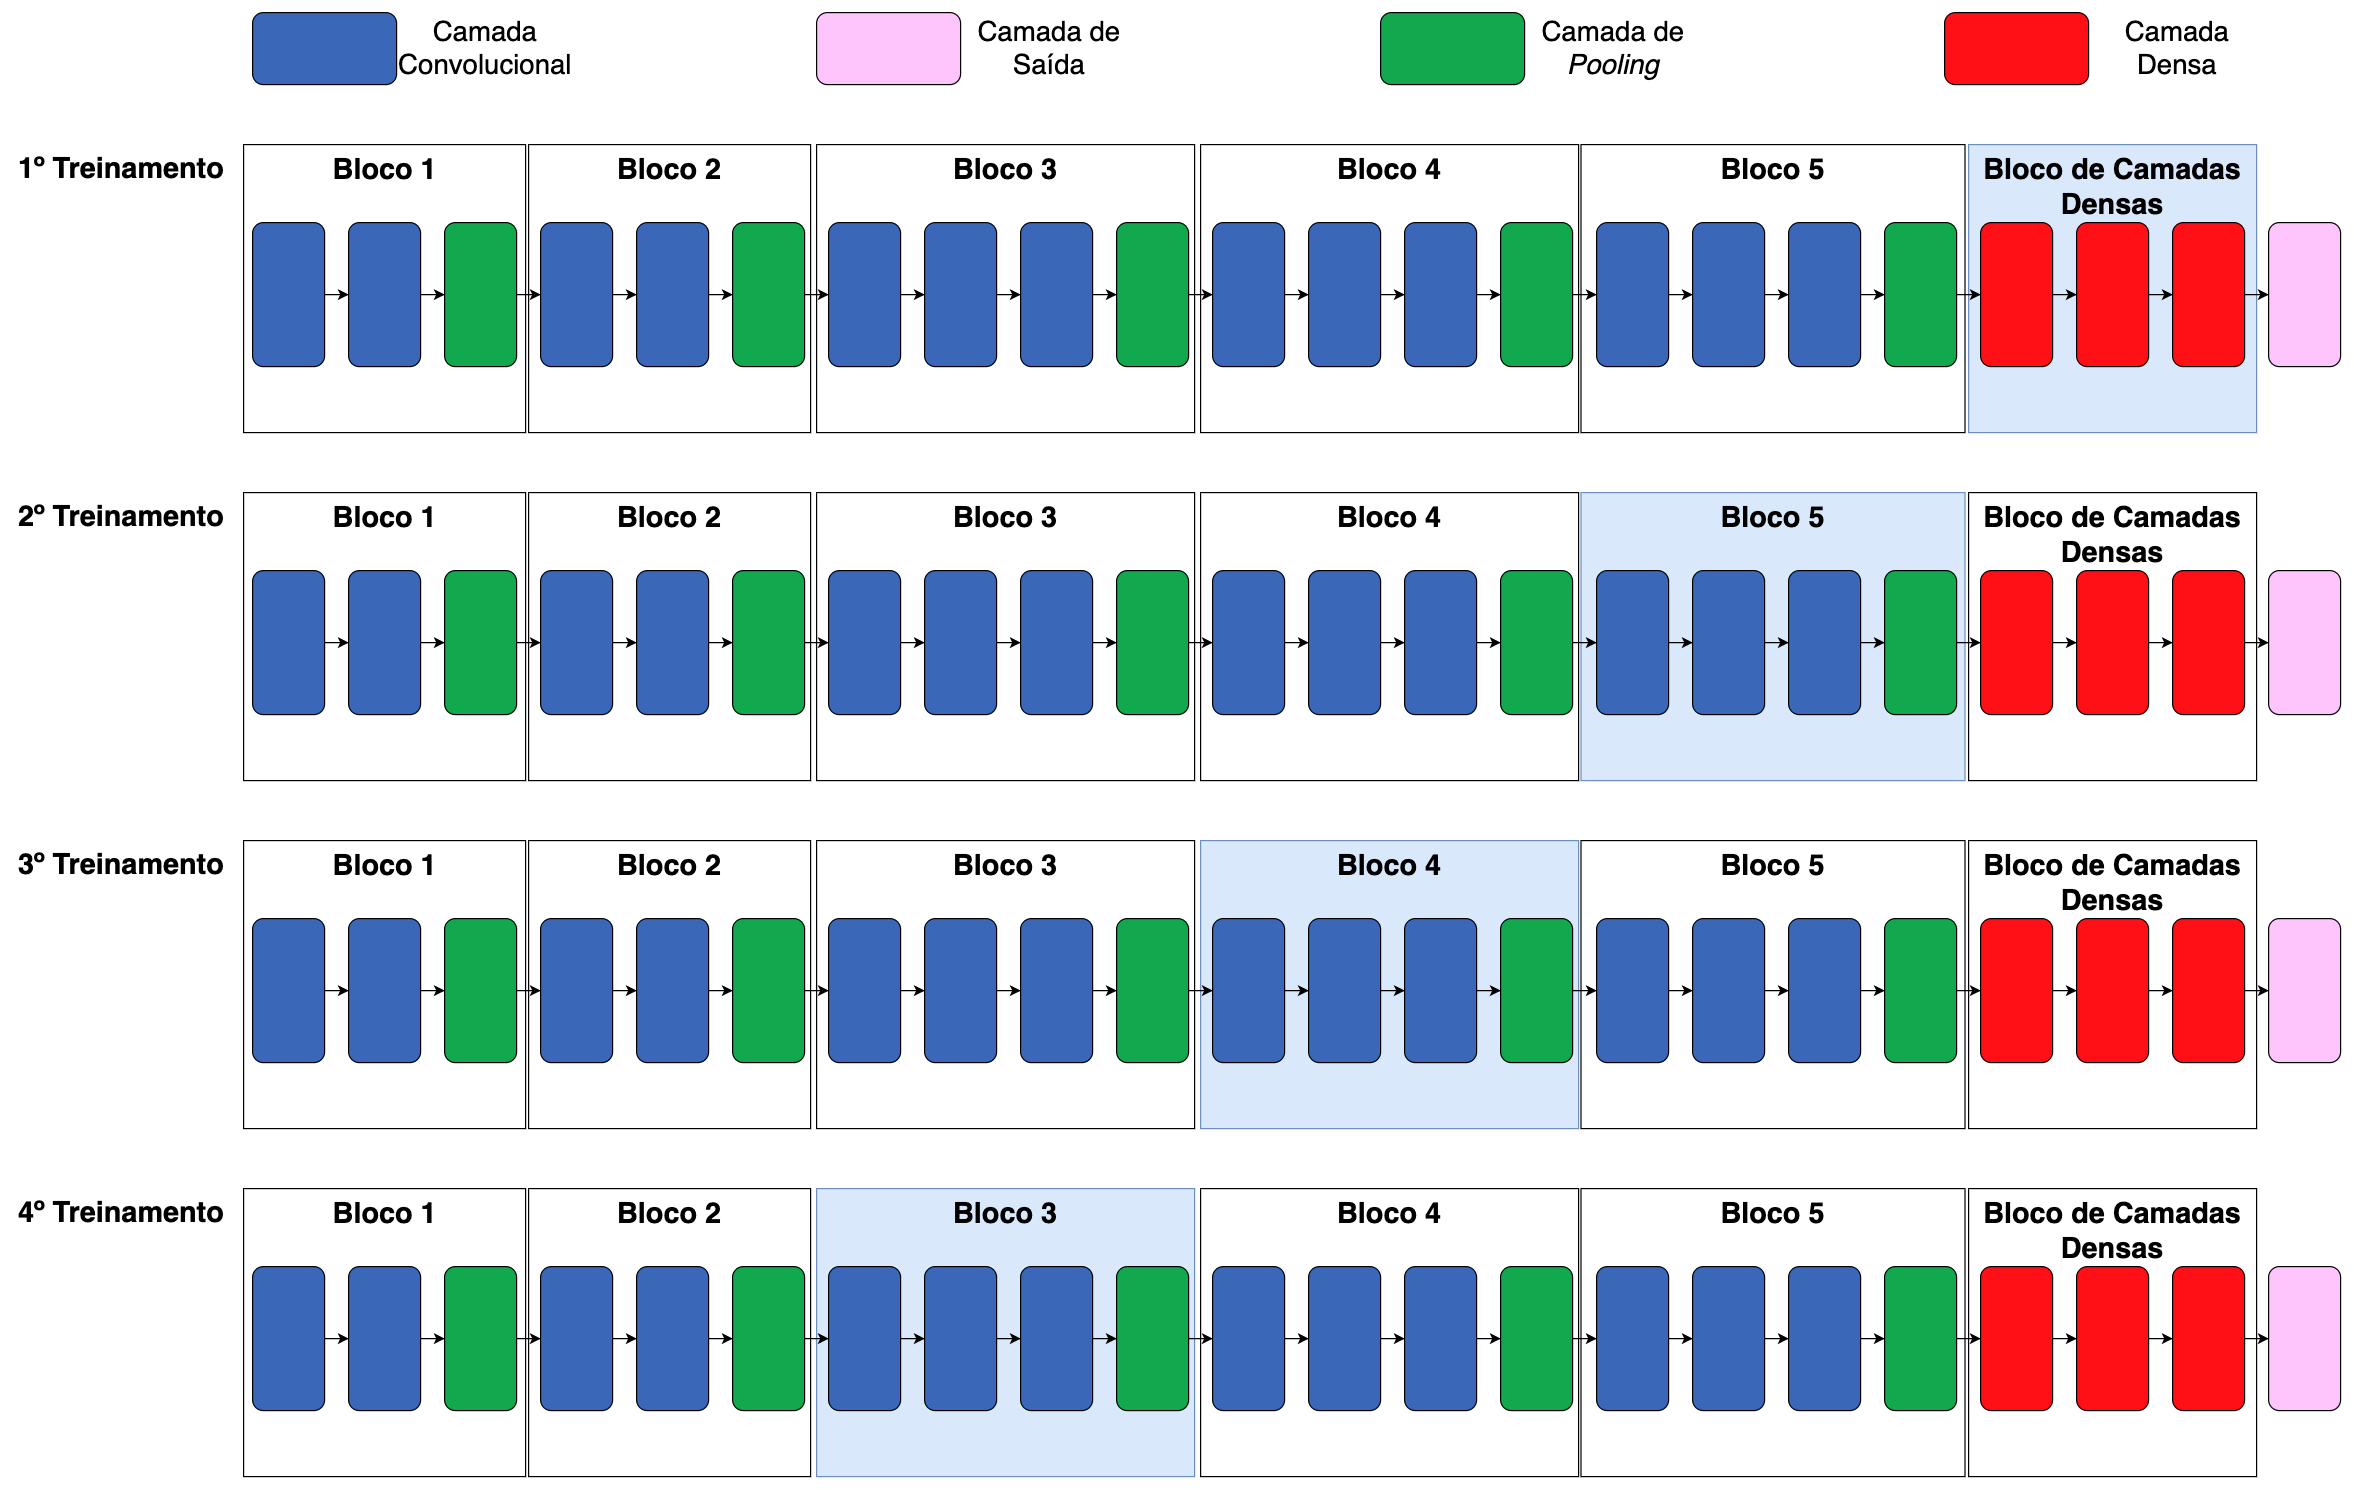
\includegraphics[width=1\textwidth]{recursos/imagens/project/fine-tunning.png}
    \label{project:fig:transf1}

    Fonte: do próprio autor.
\end{figure}

No que tange aos testes efetuados com os modelos U-Net e U-Net-Like, é relevante salientar que não se empregou as técnicas de transferência de aprendizado, devido a alguns aspectos cruciais da própria técnica. O primeiro desafio é a necessidade de utilizar a mesma arquitetura para o modelo de base adotado para a transferência de aprendizado e para o modelo treinado. Ainda que soluções para essa questão tenham sido propostas, como a adoção de camadas da VGG-16 dentro da estrutura de uma U-Net \citep{Pravitasari2020UNet-VGG16Segmentation}, a aplicação de tal técnica poderia afetar os resultados pretendidos decorrentes exclusivamente da modificação da camada de \textit{pooling} nos modelos U-Net e U-Net-Like. Adicionalmente, a escassez de conjuntos de dados robustos, similares ao ImageNet, direcionados ao processo de segmentação semântica, configura outro obstáculo, especialmente considerando a falta de padronização no formato das anotações. Como referência para um adequado conjunto de dados e modelo de anotação, podemos citar o COCO-\textit{stuff} \citep{Caesar2016} e o formato de anotação COCO, que pode ser desenvolvido a partir da ferramenta \textit{COCO Annotator} \citep{Brooks2019COCOAnnotator}.

\subsubsection{Aumento de Dados}
\label{project:augment}

\paragraph{VGG-16}

\paragraph{U-Net-Like}

\paragraph{U-Net}

\subsubsection{Parâmetros de Treinamento e Teste}
\label{project:params}


\subsubsection{Alteração na Camada de \textit{Pooling}}
\label{project:change_pooling}


\paragraph{VGG-16}

\paragraph{U-Net-Like}

\paragraph{U-Net}

Como explicado na Seção \ref{cnn:pooling}, a adaptação dos modelos de \textit{pooling} é crescente, sendo que essas modificações são motivadas pelos problemas a serem resolvidos, sendo assim, quando se trata de segmentações modernas, duas abordagens ganham destaque como técnicas de \textit{pooling}, sendo elas:

Entretanto, vale citar que, no presente trabalho, além da escolha dos modelos acima listados, também será realizado um experimento com a aplicação da técnica de \textit{Block-Based Principal Component Analysis} (ou BPCA) nas camadas de \textit{pooling} dos modelos base para a realização da segmentação panóptica. O BPCA, desenvolvido por Salvadeo \textit{et al.} \cite{Salvadeo2011}, que se provou satisfatório para aplicações relacionadas ao reconhecimento de faces, realiza a aplicação do método \textit{Principal Component Analysis} (PCA) entre blocos que dividem uma imagem original, de modo a manter as estruturas espaciais da imagem original. Sendo assim, para o presente trabalho, tem-se a expectativa de adicionar esse método na camada de \textit{pooling} do modelo base  de segmentação panóptica ciente de parte, tendo uma redução de dimensionalidade e mantendo as estruturas originais da entrada em questão, o que normalmente é perdido quando se aplica uma estratégia de \textit{pooling} em escala global (como representado nas Figuras \ref{cnn:fig:gmax_pooling} e \ref{cnn:fig:gmax_pooling} ).  Um exemplo desse módulo pode ser visualizado na Figura \ref{project:pcapooling:fig:3}.

\begin{figure}[H]
    \centering
    \caption{Exemplo representativo do processo do BPCA.}
    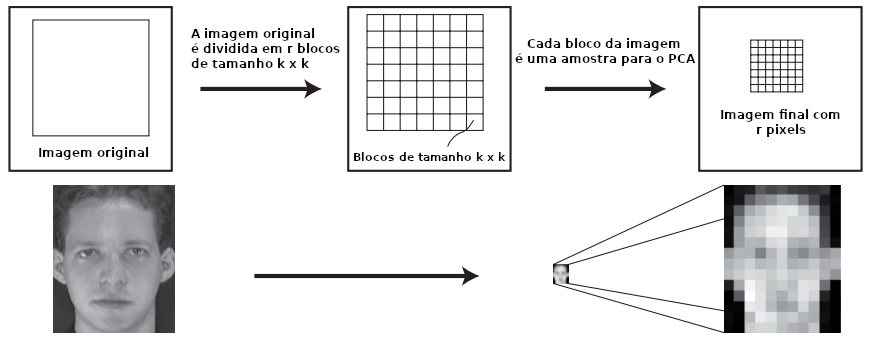
\includegraphics[width=1\textwidth]{recursos/imagens/project/BPCA.png}
    \label{project:pcapooling:fig:3}

    Fonte: retirado e adaptado de \cite{Salvadeo2011}.
\end{figure}

\subsection{Metodologia Experimental}
\label{project:exp_result}
O método de avaliação escolhido seguiu no mesmo caminho do artigo tomado como referência para realizar a segmentação \textit{Part-Aware Panoptic Segmentation} \cite{DeGeus2021}, que, no que lhe concerne, teve como base o artigo pioneiro de segmentação panóptica \cite{Kirillov2019a}, que aplica a métrica PQ (Equação \ref{panoptic:eq:2}), realizando uma sucinta adaptação que possibilita quantificar as partes das segmentações panópticas visto que é aplicado para cada uma das classes ($l$) presentes na cena, sendo elas \textit{thing} ou \textit{stuff}. Através da equação \ref{project:avaliation:eq:1} é possível entender a métrica de avaliação \textit{Part-PQ}, a qual fora escolhida para avaliação:

\begin{equation}
\label{project:avaliation:eq:1}
    PartPQ = \frac{\sum _{(p,g) \in VP} IoU_p(p,g)}{|VP|+ \frac{1}{2}|FP| + \frac{1}{2}|FN|}.
\end{equation}

Em relação à Equação \ref{project:avaliation:eq:1}, destaca-se ainda que a segmentação das partes dentro de um segmento é capturada principalmente por meio do termo $IoU_p(p,g)$, sendo que no termo é aplicado um condicional com o intuito de deixar a classe segmentada com parte ($\mathcal{L}^{parts}$) e sem partes ($\mathcal{L}^{no-parts}$) dentro das mesmas condições, ou seja, para as classes com partes presentes, aplica-se a métrica de $mIoU$ para cada pixel de parte dentro de um segmento, enquanto para segmentações sem partes, aplica-se a $IoU$ que comumente é utilizada na métrica PQ (Equação \ref{panoptic:eq:2}). O condicional supracitado dá-se por meio da seguinte expressão:

\begin{equation}
\label{project:avaliation:eq:2}
    IoU_p(p,g)= \left\{\begin{matrix}
        mIoU_{part}(p,g), & l \in \mathcal{L}^{parts}    & \\ 
        IoU_{ins}(p,g),        & l \in \mathcal{L}^{no-parts} & 
    \end{matrix}\right.
\end{equation}

Por fim, após a aplicação de PartPQ em todas as classes, calcula-se a média entre avaliações realizadas, de modo que é possível avaliar o desempenho do modelo em toda a cena e demonstrou resultados consideráveis quando comparado à métrica original \cite{DeGeus2021}.

\subsubsection{Comportamento das Métricas}

\subsubsection{Explicação de Modelos}


\subsection{Revisão de Literatura}
\label{project:revision}
Em meio a vários estilos de revisão, vale dizer que a revisão sistemática é amplamente difundida em meio cientifico, destacando-se em pesquisas de âmbito clínico e médico e garantindo menos viés, maior confiabilidade e um resumo de forma crítica dos trabalhos científicos \cite{barbosa2019}. Sendo assim, no presente trabalho, foi realizada uma revisão, bem como buscas baseadas nos artigos \cite{barbosa2019} e \cite{liberati2009}, de modo que se inspirou nas recomendações dos mesmos, salvo os casos relacionados a questões de aplicações clínicas.

Em relação às revisões, foram realizadas duas, de modo a abranger tanto os artigos técnicos em relação à segmentação panóptica, quanto artigos que servissem de base para a segmentação na área odontológica. A questão a ser tomada como base para esse estudo é: Como projetar um arcabouço para segmentar imagens de componentes visuais hierarquicamente?

Para a primeira revisão citada, foram procurados todo tipo de estudo publicados a partir do ano de 2019 até o ano presente (2022) com o assunto relacionado a \textit{panoptic segmentation}, de modo a se basear no ano de publicação do artigo pioneiro \cite{Kirillov2019a} no assunto. Foram usados os termos a seguir em diferentes combinações: ``\textit{panoptic segmentation}'', ``\textit{part}'' e ``\textit{part-aware}''. Os idiomas foram restritos à português e inglês.

O critério de inclusão baseou-se em artigos que possuíssem a citação da técnica de segmentação \textit{part-aware}, de modo a contribuir com uma segmentação hierárquica dos componentes que compunham a cena. Já em relação aos critérios de exclusão destaca-se artigos com descrição inadequada em relação ao interesse dessa revisão. Quando o artigo era específico para uma determinada aplicação que não condizia com o tema (como carros autônomos) e quando o estudo estava duplicado entre as ferramentas de busca.

Sendo assim, os indicadores referentes às pesquisas realizadas sobre esse assunto podem ser visualizadas no diagrama abaixo (Figura \ref{project:revision:fig:1}).

\begin{figure}[H]
    \centering
    \caption{Diagrama de revisão de estudos em segmentação panóptica.}
    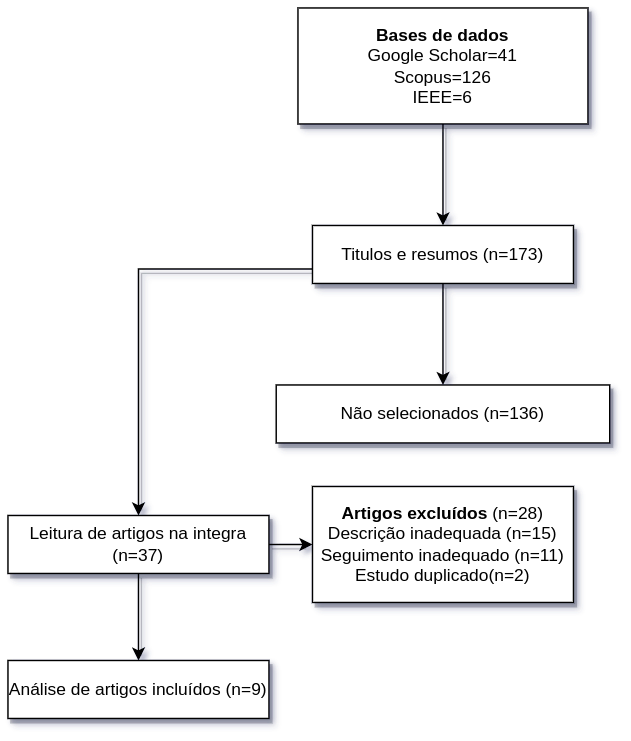
\includegraphics[height=4.5in]{recursos/imagens/project/revisao_panoptica.png}
    \label{project:revision:fig:1}

    Fonte: do próprio autor.
\end{figure}

Sendo assim, por meio do estudo realizado em relação às referências de segmentação panóptica apenas nove foram escolhidos, para complementar o presente estudo, como demonstrado na Figura \ref{project:revision:fig:1}, os quais são listados na Tabela \ref{project:revision:tab:1}.

\begin{table}[H]
    \centering
    \caption{Trabalhos selecionados a partir da revisão sobre segmentação panóptica.}
    \label{project:revision:tab:1}
    \resizebox{\textwidth}{!}{
    \begin{tabular}{l|l}
        \textbf{Título}                                                &  \textbf{Referência}    \\ \hline
        Part-Aware Panoptic Segmentation                               &  \cite{DeGeus2021}      \\
        Improving Panoptic Segmentation at All Scales                  &  \cite{Porzi2021}       \\
        SpatialFlow: Bridging All Tasks for Panoptic Segmentation      &  \cite{Chen2019a}       \\
        Visual relation of interest detection based on part detection  &  \cite{YouZhou2021}     \\
        Panoptic Image Annotation with a Collaborative Assistant       &  \cite{Jasper2020}      \\
        Panoptic Segmentation-Based Attention for Image Captioning     &  \cite{Cai2020}         \\
        Supplementary Material: Part-aware Panoptic Segmentation       &  \cite{DeGeus2021a}     \\
        Panoptic Segmentation: A Review                                &  \cite{Elharrouss2021}  \\
        PartImageNet: A Large, High-Quality Dataset of Parts           &  \cite{He2021}   
    \end{tabular}}

    \vspace*{1 cm}
    Fonte: do próprio autor.
\end{table}

Quando se trata da segunda revisão em pauta, a que contempla as segmentações na área odontológica, destaca-se que os estudos procurados também não se limitaram ao tipo, incluindo congressos, artigos de revista, entre outros, além de utilizarem o intervalo dos anos de 2019 a 2022 como métrica, de modo a encontrar segmentações odontológicas que acompanhassem a técnica de segmentação panóptica. Os termos utilizados estão listados a seguir, de modo que foram buscados em diferentes combinações: ``odonto'', ``\textit{dentistry}'', ``\textit{deep learning}'', ``\textit{semantic segmentation}'', ``\textit{instance segmentation}'', ``\textit{panoptic segmentation}'' e ``CNN''. Os idiomas foram restritos à português e inglês.

Quanto aos critérios de inclusão, destaca-se os artigos que abordaram ao menos uma das segmentações modernas, de feitio a estarem alinhados com a proposta do projeto. Quanto aos critérios de exclusão, pode-se dizer que são similares aos da primeira revisão, relatando artigos com descrição inadequada acerca da revisão em questão, estudos duplicados entre as ferramentas de busca e quando o estudo não estava diretamente relacionado aos temas ``segmentação'' e ``odontologia''. Dessa forma, por meio da Figura \ref{project:revision:fig:2} é possível visualizar a representação da revisão realizada.

\begin{figure}[H]
    \centering
    \caption{Diagrama de revisão de estudos em segmentação odontológica.}
    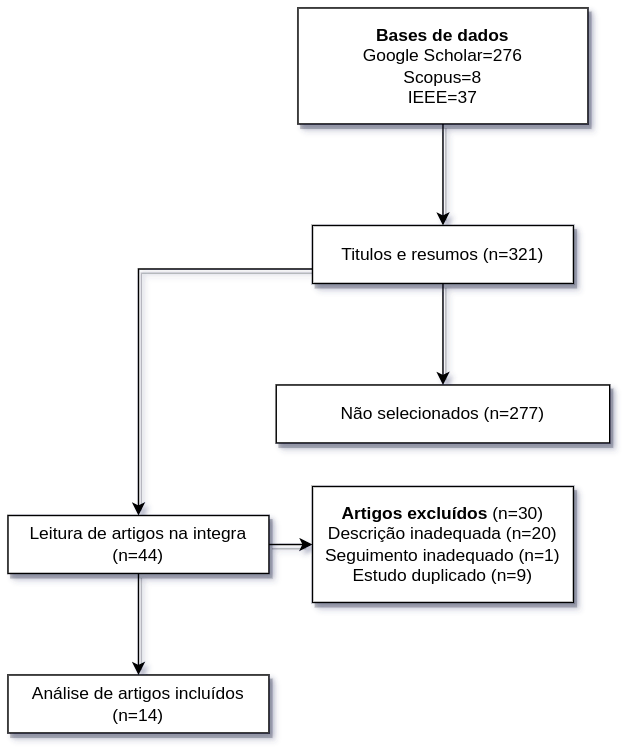
\includegraphics[height=4.5in]{recursos/imagens/project/revisao_odonto.png}
    \label{project:revision:fig:2}


    Fonte: do próprio autor.
\end{figure}

Tendo em vista os estudos que estão relacionados à segmentação na área odontológica, destacando aqueles que fazem uso das segmentações modernas (semântica, de instâncias ou panóptica), por meio da Figura \ref{project:revision:fig:2} cita-se que apenas 14 foram determinados como relevantes, os quais são listados na Tabela \ref{project:revision:tab:2}.

\begin{table}[H]
    \centering
    \caption{Trabalhos selecionados a partir da revisão sobre segmentação odontológica.}
    \label{project:revision:tab:2}
    \resizebox{\textwidth}{!}{
    \begin{tabular}{l|l}
        \textbf{Título}                                                                                                              &  \textbf{Referência}  \\ \hline
        A study on tooth segmentation and numbering using end-to-end deep neural networks                                            &  \cite{Silva2020}       \\
        Accurate Segmentation of Dental Panoramic Radiographs with U-NETS                                                            &  \cite{Koch2019}        \\
        ToothNet: Automatic Tooth Instance Segmentation and Identification From Cone Beam CT Images                                  &  \cite{Cui2019}         \\
        Toothpix: Pixel-Level Tooth Segmentation in Panoramic X-Ray Images based on Generative Adversarial Networks                  &  \cite{Cui2021}         \\
        Simultaneous Nuclear Instance and Layer Segmentation in Oral Epithelial Dysplasia                                            &  \cite{Shephard2021}    \\
        Automated detection and classification of oral lesions using deep learning to detect oral potentially malignant disorders    &  \cite{Tanriver2021}    \\
        Pose-aware instance segmentation framework from cone beam CT images for tooth segmentation                                   &  \cite{Minyoung2020}    \\
        Mask-MCNet: Instance Segmentation in 3D Point Cloud of Intra-oral Scans                                                      &  \cite{Ghazvinian2021}  \\
        Artificial Intelligence for Fast and Accurate 3-Dimensional Tooth Segmentation on Cone-beam Computed Tomography              &  \cite{Lahoud2021}      \\
        Clinically Applicable System For 3D Teeth Segmentation in Intraoral Scans using Deep Learning                                &  \cite{Hao2020}         \\
        Machine learning in orthodontics: Challenges and perspectives                                                                &  \cite{Liu2021}         \\
        Automatic 3D tooth segmentation using convolutional neural networks in harmonic parameter space                              &  \cite{Zhang2020}       \\
        Automatic Dental Plaque Segmentation based on Local-to-global Features Fused Self-attention Network                          &  \cite{Li2022}          \\
        Interpretable and Interactive Deep Multiple Instance Learning for Dental Caries Classification in Bitewing X-rays            &  \cite{Bergner2021}  
    \end{tabular}}

    \vspace*{1cm}
    Fonte: do próprio autor.
\end{table}

\subsection{Considerações Finais do Capítulo}